\par Zaproponowany system komputerowy charakteryzuje się następującymi cechami:
				
				\begin{itemize}
					\item Bezpieczeństwem przechowywania danych
					\item Niezawodnością
					\item Wydajnością
					\item Pojemnością
				\end{itemize}
		
				\subsubsection{Bezpieczeństwo przechowywania danych}
					Aby zadbać o bezpieczeństwo danych należy przedsięwziąć odpowiednie kroki zmierzające do ich ochrony:
				
					\begin{description}
					
						\item[\textbf{Redundancja danych}] Zabezpieczenie polegające na przechowywaniu danych w dwóch kopiach. Wszystkie istotne dane pojawiające się w systemie przechowujemy wraz z kopią zapasową. Co najistotniejsze, kopia ta tworzona jest w czasie rzeczywistym. Dzięki temu potrzebne dane chronione są od momentu powstania.
				
						\item[\textbf{Utrzymanie wersji produkcyjnej i rozwojowej}] Strategia ta zakłada utrzymanie wersji rozwojowej i produkcyjnej oprogramowania, zarówno w zakresie sklepu internetowego jak i systemu zarządzania. Wszystkie zmiany w funkcjonowaniu sklepu muszą zostać wprowadzone najpierw na wersji rozwojowej, gdzie zostaną gruntownie przetestowane, a dopiero po zatwierdzeniu wprowadzane do wersji produkcyjnej. 
						
						\item[\textbf{Zabezpieczenie baz danych}] Dla bazy danych sklepu internetowego i systemu zarządzania należy skonfigurować PITR (Point In Time Recovery), powrót do punktu w czasie. Jest to rozwiązanie wykorzystywane np. przy systemach przeprowadzających operacje finansowe. W razie awarii możliwe jest odtworzenie stanu systemu z dokładnej daty sprzed awarii. Mechanizm ten zapisuje historię operacji wykonywanych na bazie danych wraz z dokładną datą. Dzięki temu bazę danych zabezpieczoną tym mechanizmem można odtwarzać operacja po operacji.

					\end{description}
					
			\subsubsection{Niezawodność}
					\par Celem analizy niezawodności systemu komputerowego należy zaznajomić się ze statystykami awaryjności sprzętu elektronicznego. Pierwszy wykres przedstawia statystyki awaryjności sprzętu produkowanego przez danego producenta. Wykres ten pozwala ustalić średnią awaryjność w ciągu pierwszego, drugiego i trzeciego roku użytkowania sprzętu, oraz trzyletniego czasu użytkowania. 
				
					\begin{figure}[H]
						\centering
						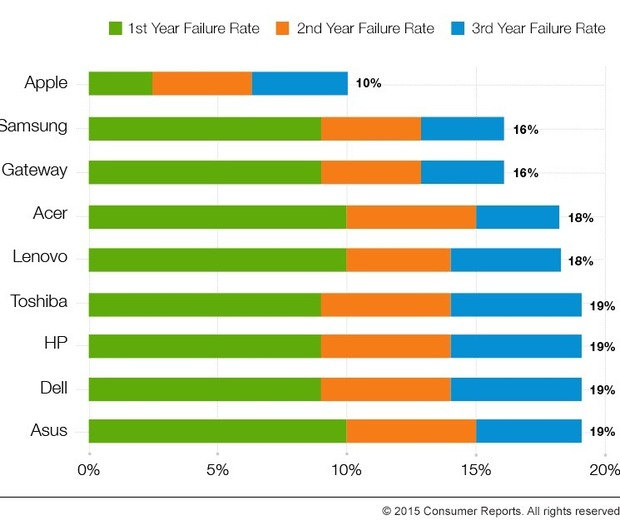
\includegraphics[scale=0.35]{consumer_reports_failures}
						\caption{Raport awaryjności sprzętu elektronicznego}
						\label{rep_fail}
					\end{figure}
				
				\par Na podstawie wykresu \ref{rep_fail} można określić, że prawdopodobieństwo awarii w pierwszym roku wynosi ok. 8 \%, a w roku drugim i trzecim ok. 5\%. Na tej podstawie można stwierdzić, że 20\% zakupionego sprzętu elektronicznego zepsuje się w przeciągu 3 lat użytkowania. Należy zapoznać się również z tzw. "krzywą wanny" prezentującą awaryjność sprzętu elektronicznego. Można odczytać z niej bardzo istotne informację. Pierwszy obszar wykresu obejmuje początek cyklu życia produktu. Prawdopodobieństwo awarii produktu w tym obszarze jest największe na początku cyklu i spada po krzywej hiperbolicznej aż do ustabilizowania się w etapie drugim. Na pierwszym etapie duża awaryjność jest powodowana błędami w produkcji, prześliźnięciem się produktu przez kontrolę jakości itp. Na drugim etapie mamy stały odsetek awarii sprzętowych. Wynika to ze zwykłej losowości i praw Murphy'iego - rzeczy się psują. Na końcowym etapie życia produktu krzywa awarii znów przybiera postać hiperboli i dość szybko zmierza ku górze. Na tym etapie podatność na awarię wzrasta i wynika ona z takich czynników jak: zużycie, zmęczenie materiałów itp. Należy pamiętać, że elementy użyte w sprzęcie mają określoną ilość godzin pracy, cykli odczytu/zapisu itp. lub zostały zaprojektowane z takich materiałów, aby popsuły się po okresie gwarancyjnym. 
				
				\begin{figure}[H]
					\centering
					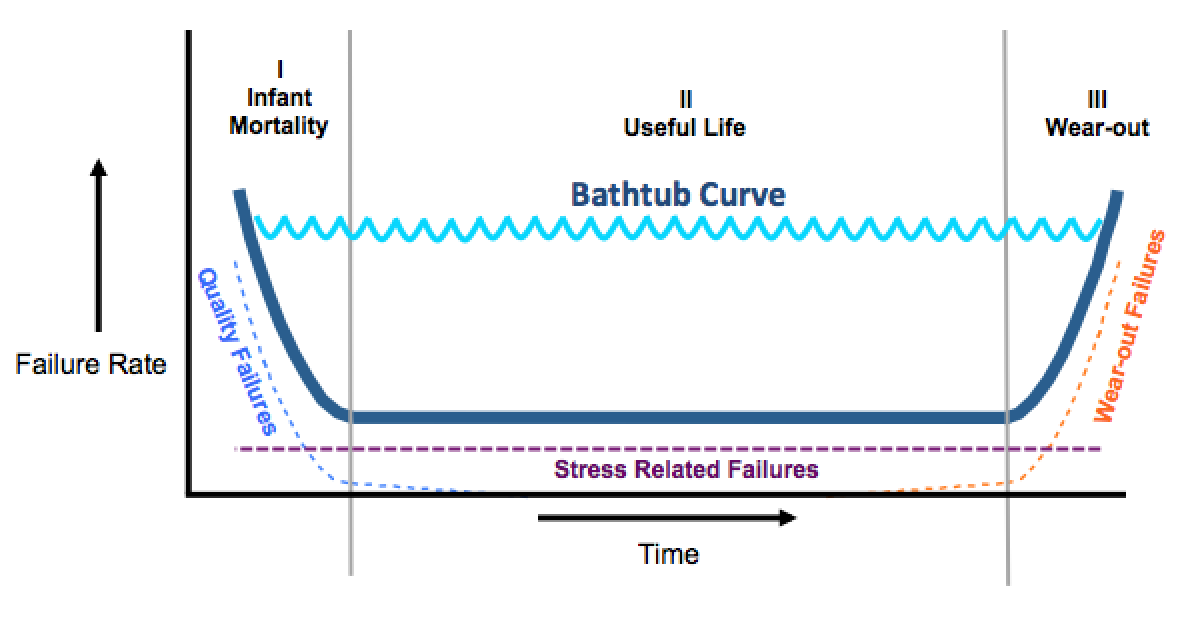
\includegraphics[scale=0.35]{bath_curve}
					\caption{Krzywa wanny prezentująca awaryjność sprzętu}
				\end{figure}

				\par Niezawodności należy rozpatrywać pod katem dwóch przypadków. Pierwszym z nich jest niezawodność programowa, drugą zaś niezawodność sprzętowa platformy. W jednym i drugim przypadku, rozwiązaniem jest duplikacja elementów systemu wykonujących te same zadania. Koncepcję tą z powodzeniem można wytłumaczyć odwołując się do rozkładu dwumianowego, nazywanego też schematem Bernoulli'ego.
				
				\[ P_n(k) = \binom{n}{k} p^k (1-p)^{n-k} \]
			
				gdzie:
			
				\begin{description}
					\item n - ilość prób 
					\item k - ilość sukcesów 
					\item p - prawdopodobieństwo sukcesu
				\end{description}
				
				Wzór ten opisuje nam prawdopodobieństwo uzyskania "k" sukcesów w "n" próbach. Przyjmując jako "sukces" wystąpienie awarii można policzyć niezawodność systemu. 
			
				\begin{enumerate}
					\item W przypadku jednego urządzenia wykonującego dane zadanie należy wziąć pod uwagę uśrednione dane z histogramu:
							\begin{itemize}
								\item Prawdopodobieństwo awarii w pierwszym roku wynosi 8\%, w drugim i trzecim 5\%
								\item Prawdopodobieństwo awarii przez cykl 3 lat wynosi 18%
							\end{itemize}
					\item w przypadku dwóch urządzeń realizujących tą samą funkcję, zakładając że wystarczy jeden z nich otrzymujemy:
							\begin{itemize}
								\item Prawdopodobieństwo awarii w pierwszym roku \( P_2(2) = \binom{2}{2} 0.08^2 (1-0.08)^{2-2} = 0.0064*100\% = 0.64\%\)
								\item Prawdopodobieństwo awarii w drugim i trzecim roku \( P_2(2) = \binom{2}{2} 0.05^2 (1-0.05)^{2-2} = 0.0025*100\% = 0.25\%\)
								\item Prawdopodobieństwo awarii przez cykl 3 lat wynosi \( P_2(2) = \binom{2}{2} 0.18^2 (1-0.18)^{2-2} = 0.0324*100\% = 3.24\%\)
								\item Prawdopodobieństwo awarii jednego z dwóch urządzeń przez cykl 3 lat wynosi \( P_2(1) = \binom{1}{2} 0.18^1 (1-0.18)^{2-1} = 0.2952*100\% = 29.52\%\)
							\end{itemize}
				\end{enumerate}
				
				\par Jak wynika z przeprowadzanych rozważań, celem ochrony danych oraz logicznej separacji systemu komputerowego, należy rozdzielić elementy przetwarzające oraz przechowujące dane. Celem osiągnięcia pożądanej jak najniższej awaryjności, należy podzielić system komputerowy na dwie grupy. Pierwszą z nich będzie grupa przetwarzająca dane a druga będzie grupą przechowującą dane. Z przeprowadzonych obliczeń wynika, że prawdopodobieństwo awarii krytycznej w każdej grupie wynosi 3.24\%. Na tej podstawie, dla 3 letniego cyklu użytkowania sprzętu, można wysnuć następujące wnioski:
				
				\begin{itemize}
					\item Prawdopodobieństwo awarii krytycznej tzn. uniemożliwiającej dalszą pracę systemu wynosi 3.24\% w czasie 3 lat
					%\item Prawdopodobieństwo awarii krytycznej całego systemu wynosi 0.1\% 
					\item Prawdopodobieństwo awarii nie krytycznej tzn. wpływającej jedynie na wydajność systemu wynosi 8.71\% w okresie roku i 29.52\% w okresie 3 lat
				\end{itemize}
			
			\subsubsection{Wydajność}
				\par Celem zapewnienia optymalnego przetwarzania żądań system komputerowy musi charakteryzować się wydajnością rozumianą jako zestaw parametrów określających jego możliwości. Tymi parametrami są ilość rdzeni procesora oraz rozmiar pamięci operacyjnej. Poniższa lista prezentuje minimalne parametry jakie muszą posiadać serwery, aby przetwarzanie danych było możliwe. 
				
				\begin{itemize}	
						\item{\textbf{serwer DNS}} Wystarczające będzie zarezerwowanie 1 rdzenia procesora i 2GB pamięci operacyjnej, ze względu na wykonywania nieskomplikowanych zadań jakimi jest tłumaczenie nazw mnemonicznych na adresy sieciowe.
						
						\item{\textbf{serwer E-Mail}} Ze względu na filtrowanie wirusowe i filtrowanie spamu, czyli niechcianej poczty. Należy na niego zarezerwować 2 rdzenie procesora oraz 4GB pamięci operacyjnej.
						
						\item{\textbf{serwer Baz danych}} Wydajność pozostałych systemów zależy od szybkości realizacji zapytań na bazach danych, serwer ten musi być wydajny. Ze względu na to zarezerwowane dla niego zostaną 4 rdzenie procesora, oraz 4 GB pamięci operacyjnej.
						
						\item{\textbf{centrala telefoniczna}} Ze względu na nagrywanie rozmów, bezpieczne będzie przydzielenie tu 3 rdzeni procesora oraz 4 GB pamięci operacyjnej. 
						
						\item{\textbf{współdzielony system plików}} Musi posiadać on co najmniej 2 rdzenie procesora i 8 GB pamięci operacyjnej na pamięć pośrednią otwartych plików, oraz ze względu na to, że jego wydajność jest kluczowa dla działania wszystkich innych podsystemów.
						
						\item{\textbf{serwer www}}  Ze względu na konieczność generowania dynamicznej strony internetowej przygotowanej w języku skryptowym, oraz świadczenie jej klientom za pomocą serwera http. Wymagać to będzie co najmniej 2 rdzeni procesora i co najmniej 4GB pamięci operacyjnej.
					
					\end{itemize}	
			
					Po przeprowadzeniu wstępnej analizy wydajnościowej udało się ustalić, że dla budowy minimalnego systemu potrzeba komputera posiadającego:
			
					\begin{itemize}
						\item 15 rdzeni procesora
						\item 28GB pamięci operacyjnej
					\end{itemize}
			
					\par Ważnym parametrem procesora jest również pamięć podręczna, nazywana z angielskiego pamięcią "cache". Odpowiada ona za magazynowanie instrukcji wykonywanych przez procesor. Instrukcje te są magazynowane w czasie gdy procesor przetwarza instrukcje wcześniej zmagazynowane. Odpowiedni dobór wielkości pamięci podręcznej pozwala na optymalne wykorzystanie technologii przetwarzania wielowątkowego. Dzięki wykorzystaniu przetwarzania wielowątkowego jeden rdzeń procesora może pracować jako dwa. Pozwoli to ograniczyć ilość rdzeni procesora dwukrotnie, z 15 do 8, jednak pociąga za sobą konieczność posiadania przez procesor co najmniej 2MB pamięci podręcznej na rdzeń fizyczny. Pozwala to określić specyfikacje komputera:
			
					\begin{itemize}
						\item 8 rdzeni fizycznych procesora
						\item 28GB pamięci operacyjnej
						\item obsługa technologii HyperThreading (przetwarzania wielowątkowego)
						\item 16MB pamięci podręcznej
					\end{itemize}
					
			\subsubsection{Pojemność}
				\par Ilość danych zależeć będzie też od funkcjonowania systemu. Głównym źródłem danych będą tu procesy związane z obsługą klienta. Poniższa lista prezentuje dane, jakie należy zabezpieczyć celem bezpiecznej realizacji procesów zamówienia i reklamacji.
	
					\begin{itemize}
						\item Zamówienie klienta
							\begin{itemize}
								\item Dane dotyczące zamówienia, pozwalające jednoznacznie określić wszystkie wymagania klienta co do tworzonego produktu.
								\item Zlecenie produkcji przesyłane do producenta będące specyfikacją wedle której wykonany ma zostać dany produkt.
								\item Dokumenty powstałe w procesie zamówienia tj. faktury, paragony, dokumenty transportowe, kopie paragonów.
							\end{itemize}
						\item Reklamacja klienta
							\begin{itemize}
								\item Zdjęcia uszkodzonego produktu i zgłoszenie reklamacji.
								\item Dokumenty powstałe w procesie reklamacji tj. faktury, dokumenty transportowe, decyzja.
							\end{itemize}
						\item Rozmowy telefoniczne
							\begin{itemize}
								\item Rozmowy telefoniczne z klientami.
								\item Rozmowy telefoniczne z producentami.
							\end{itemize}
					\end{itemize}
		
					\par Dla obliczenia ilości, należy ustalić parametry, związane z wymienionymi wcześniej czynnościami i procesami. Określenie ich niezbędne jest do oszacowania ilości danych zbieranych podczas obsługi klientów i funkcjonowania sklepu. 
		
					\begin{itemize}
						\item Zmienne globalne 
							\begin{description}
								\item \( R_z \) średni rozmiar zdjęcia
								\item \( Z_r \) przewidywana ilość zamówień rocznie
								\item \( L_p \) wymagane lata przechowywania danych
								\item \( H_m \) średni rozmiar wiadomości e-mail
								\item \( C_r \) średni rozmiar minuty rozmowy
								\item \( D_s \) średni rozmiar jednego dokumentu
								\item \( R_r \) współczynnik reklamacji
							\end{description}
						\item Zmienne określające parametry potrzebne do wyliczenia ilości danych potrzebnych na informacje o produktach od producentów
							\begin{description}
								\item \( M_p \) średnia ilość mebli od producenta
								\item \( Z_p \) średnia ilość zdjęć na produkt
								\item \( P_w \) ilość współpracujących producentów
							\end{description}
						\item Zmienne określające parametry potrzebne do wyliczenia ilości danych potrzebnych na prawidłowe zabezpieczenie procesu zamówienia
							\begin{description}
								\item \( O_z \) średnia ilość zdjęć na zamówienie 
								\item \( L_z \) średnia ilość zdjęć z produkcji 
							\end{description}
						\item Zmienne określające parametry potrzebne do wyliczenia ilości danych potrzebnych do utrwalenia komunikacji
							\begin{description}
								\item \( X_r \) średni czas rozmowy telefonicznej w minutach
								\item \( M_c \) średnia ilość pozostałych wiadomości e-mail dziennie
								\item \( K_l \) średnia ilość telefonów na zamówienie
								\item \( T_p \) średnia ilość wiadomości e-mail na zamówienie
							\end{description}
						\item Zmienne określające ilość zużytych danych od przechowywanych dokumentów
							\begin{description}
								\item \( D_z \) średnia ilość dokumentów powstałych w procesie zamówienia
							\end{description}
						\end{itemize}
		
						\par Kolejnym krokiem jest wyznaczenie funkcji opisujących ilość powstałych danych od czynności wykonanych w procesach i czynników takich jak ilość producentów i zamówień.
		
						\begin{itemize}
							\item Zależność przedstawiająca ilość zużycia danych od ilości produktów i producentów. 
								\[  Z_{mp} = R_z \times M_p \times Z_p \times P_w \]
					
							\item Zależność przedstawiająca ilość zużycia danych od ilości zamówień
								\[ Z_{mz} = ( O_z + L_z) \times R_z \times Z_r \times L_p \]
								
							\item Zależność przedstawiająca zużycie miejsca od ilości telefonów i mail'i
								\[ Z_{km} = (Z_r \times X_r \times K_l + M_c \times H_m \times 365 + T_p \times M_c \times Z_r ) \times L_p \]
								
							\item Zależność przedstawiająca ilość zużytych danych od przechowywanych dokumentów
								\[ Z_{dm} = D_z \times D_s \times Z_r \times L_p \]
						\end{itemize}
		
						Na podstawie powyższych funkcji możemy przedstawić ilość miejsca zajętego przez dane jako sumę wcześniej ustalonych funkcji.
		
						\[ Z_a = Z_{mp} + Z_{mz} + Z_{km} + Z_{dm} \]

						Do powstałego wzoru należy doliczyć jeszcze współczynnik reklamacji. W procesie reklamacji prawdopodobnie powstanie tyle samo danych co w procesie zamówienia. Jednak procesów reklamacji będzie odpowiednio mniej niż zamówień. Aby obliczyć ilość powstałych danych, należy powiększyć dane pochodzące z obsługi sprzedaży o dane powstałe w procesie reklamacji. Przyjmując współczynnik reklamacji wyrażony w procentach można przyjąć, że ilość danych z każdej funkcji należy pomnożyć przez \( 1 + R_r \).
			
						\[ Z_a = Z_{mp} + (1 + R_r) \times Z_{mz} + (1 + R_r) \times (1 + R_r) \times Z_{km} + (1 + R_r) \times Z_{dm} \]
			
						Pamiętajmy o zastosowaniu technologii redundancją danych na wypadek awarii, dzięki czemu wszystko przechowujemy w dwóch kopiach 
						
						\[ Z_a = 2 \times ( Z_{mp} + (1 + R_r) \times Z_{mz} + (1 + R_r) \times Z_{km} + (1 + R_r) \times Z_{dm} ) \]
						
						Ustalmy teraz wartości zmiennych potrzebne do obliczenia ilości potrzebnego miejsca
		
						\begin{itemize}
							\item \( R_z = 1MB \)
							\item \( L_p = 5 lat \) 
							\item \( H_m = 75kB = 0.075MB \)
							\item \( C_r = 1MB/minutę \)
							\item \( D_s = 350kB = 0.35MB \)
							\item \( M_p = 10 \)
							\item \( Z_p = 5 \)
							\item \( O_z = 5 \) 
							\item \( L_z = 5 \) 
							\item \( X_r = 10 minut \)
							\item \( M_c = 4 \) 
							\item \( D_z = 8 \)
							\item \( R_r = 15\% = 0.15 \)
							\item \( K_l = 10 \)
							\item \( T_p = 10 \) 
						\end{itemize}
		
					Ustalmy również zmienne potrzebne do wyliczenia ilości potrzebnego miejsca. Jako zmienne w tym wypadku przyjęte zostały ilość zamówień rocznie oraz ilość współpracujących producentów. 
					
					\begin{itemize}
						\item \( Z_r \)
						\item \( P_w \)
					\end{itemize}
				
					Po ustaleniu stałych i zmiennych możemy przedstawić zależność jako funkcję dwóch zmiennych
				
					\[ Z_a(Z_r,P_w) = 2 \times ( Z_{mp}(P_w) + (1 + R_r) \times Z_{mz}(Z_r) + (1 + R_r) \times Z_{dm}(Z_r) + (1 + R_r) \times Z_{km}(Z_r) ) \]
				
					Podstawmy wzory funkcji
				
					\begin{equation}
						\begin{split}
							Z_a(Z_r,P_w) = 2 \times [ R_z \times M_p \times Z_p \times P_w + (1 + R_r) \times ( ( O_z + L_z) \times R_z \times Z_r \times L_p \\
							+ D_z \times D_s \times Z_r \times L_p + (Z_r \times X_r \times K_l + M_c \times H_m \times 365 + T_p \times M_c \times Z_r ) \times L_p ) ] 
						\end{split}	
					\end{equation}
					
					Po uproszczeniu
					
					\begin{equation}
						\begin{split}
							Z_a(Z_r,P_w) = 2 \times [R_z \times M_p \times Z_p \times P_w + (1 + R_r) \times L_P \times Z_r \times \\ 
							[ ( O_z + L_z) \times R_z  + D_z \times D_s + ( X_r \times K_l + M_c \times H_m \times 365 + T_p \times M_c ] ] 
						\end{split}
					\end{equation}	
					
					Podstawmy teraz ustalone wcześniej wartości. Ostatecznie funkcja przyjmuje następującą postać
					
					\begin{equation}
						\begin{split}
							Z_a(Z_r,P_w) = 100 \times P_w + 3934.5 \times Z_r
						\end{split}
					\end{equation}
					
					\begin{figure}[H]
						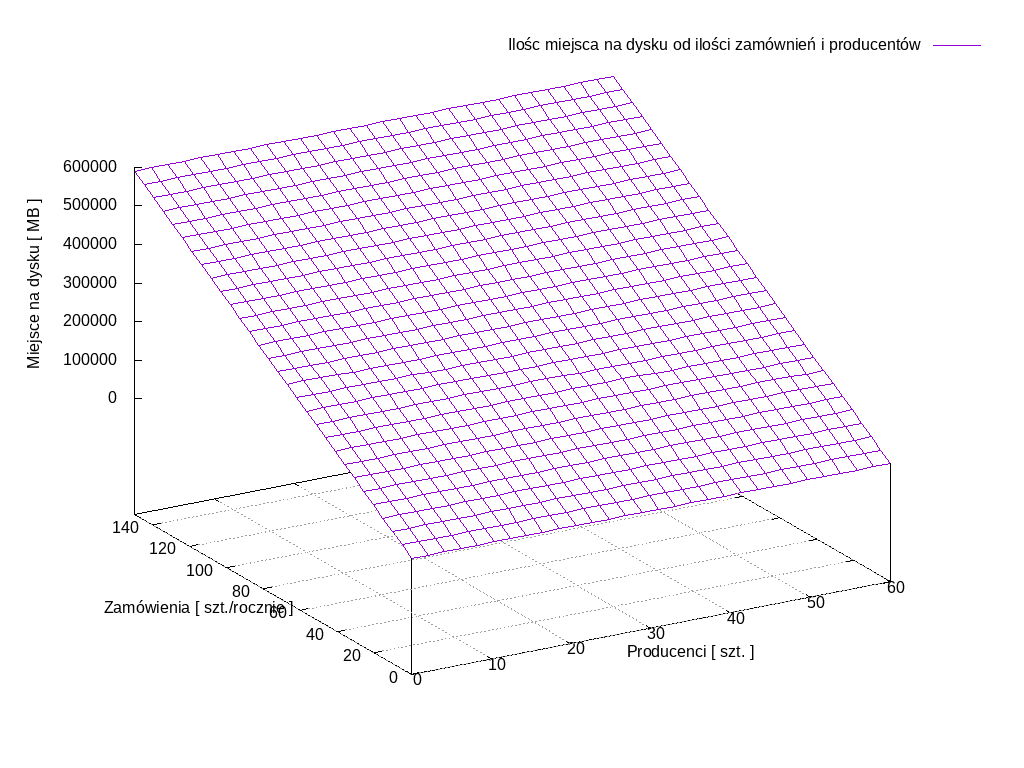
\includegraphics[scale=0.45]{storage}
						\caption{Wykres prezentujący wymaganą pojemność systemu w zależności od ilości producentów i zamówień rocznie}
					\end{figure}
				
					\par Na podstawie przygotowanej funkcji i przeprowadzonej symulacji wynika, że utrzymując około 100 zamówień rocznie i przechowując dane o działaniach z nimi związanych przez okres 5 lat, wymagane jest co najmniej 600GB pamięci. Analiza ta nie uwzględnia ilości danych pochodzących z ochrony bazy danych poprzez technologię PITR.	
 
